\documentclass[12pt]{article}
\usepackage[brazil]{babel}
\usepackage[utf8]{inputenc}
\usepackage{graphicx}

\title{Análise de características autonômicas do Google App Engine}
\author{
Herberth Amaral \\
Departamento de Ciência da Computação\\
Programa de Pós Graduação em Modelagem Computacional e Sistemas\\
Universidade Estadual de Montes Claros - UNIMONTES\\
}
\date{\today}

\begin{document}
\maketitle

\begin{abstract}
    O crescente aumento da complexidade de aplicações Web tem levado empresas a
    especializarem seus serviços e delegarem tarefas de infra-estrutura a
    outras empresas especializadas. A comum prática de configurar todo um
    ambiente de implantação de uma aplicação está sendo deixada de lado em
    favor de uma abordagem mais prática e autonômica.  Auto-cura,
    auto-otimização, auto-proteção e auto-configuração, todos elementos da
    computação autonômica, são necessários (e até exigidos) em ambientes PaaS
    (\textit{plataform as a service}), como é o caso do Google App Engine (GAE).
    Este artigo visa analisar cada um dos elementos da computação autonômica do
    GAE e mostra que ele atende satisfatoriamente todos os requisitos.
\end{abstract}

\section{Introdução}
Computação autonômica tem o objetivo de desenvolver de sistemas computacionais
capazes de auto-gerenciamento e adaptação a mudanças imprevisíveis. Alguns
serviços da World Wide Web operam em ambiente hostil e precisam responder a
mudanças de forma rápida e eficiente.

O GAE faz parte de uma nova geração de serviços conhecidos como Plataformas
Como Serviço, ou da sigla em Inglês Paas, que tem como objetivo tirar o fardo
de configuração de um abiente de implantação de aplicações web de empresas que
desenvolvem esses serviços. Com o GAE não é necessário configurar captura de
logs, auto-escala da aplicação, provisionamento de novos servidores,
armazenagem de dados e proteção contra vulnerabilidades de sistema operacional
ou da pilha de software que servirá a aplicação.

O \textit{tradeoff} imposto pelo GAE é o reduzido número de opções. Por
exemplo, não é possível acesar arquivos diretamente do sistema de arquivos, uma
vez que as instâncias são efêmeras, ou seja, podem ser destruídas a qualquer
momento. A análise detalhada dos \textit{tradeoffs} não estão no escopo deste
trabalho, entretanto.

Este trabalho tem o objetivo de analisar os componentes de computação
autonômica do GAE e está dividido nas seguintes seções: a seção 2 trata dos
detalhes do funcionamento do GAE, a seção 3 analisa as capacidades de
auto-cura, a seção 4 analisa as capacidades de auto-otimização, a seção 5
analisa as questões referentes à auto-proteção, a seção 6 analisa as
características de auto-configuração e a seção 7 delineia as considerações
finais.

\section{Detalhes de funcionamento do GAE}

Esta seção mostra a mecânica envolvida no gerenciamento de aplicações/projetos
do GAE. No geral, não há quesitos desafiadores, uma vez que os detalhes mais
complicados são gerenciados pelo próprio GAE.

\subsection{Interface com o usuário}
Com o intuito de diminuir a fricção nas configurações do ambiente da aplicação,
o GAE possui uma rica interface capaz de configurar aspectos básicos e
avançados do ambiente da aplicação. É importante notar que tais configurações
não impactam no requisito de auto-configuração dos sistemas autonômicos, pois
essas são feitas apenas uma vez. 

A figura \ref{fig:painel} mostra a interface de usuário inicial do GAE.
\begin{figure}
    \centering
    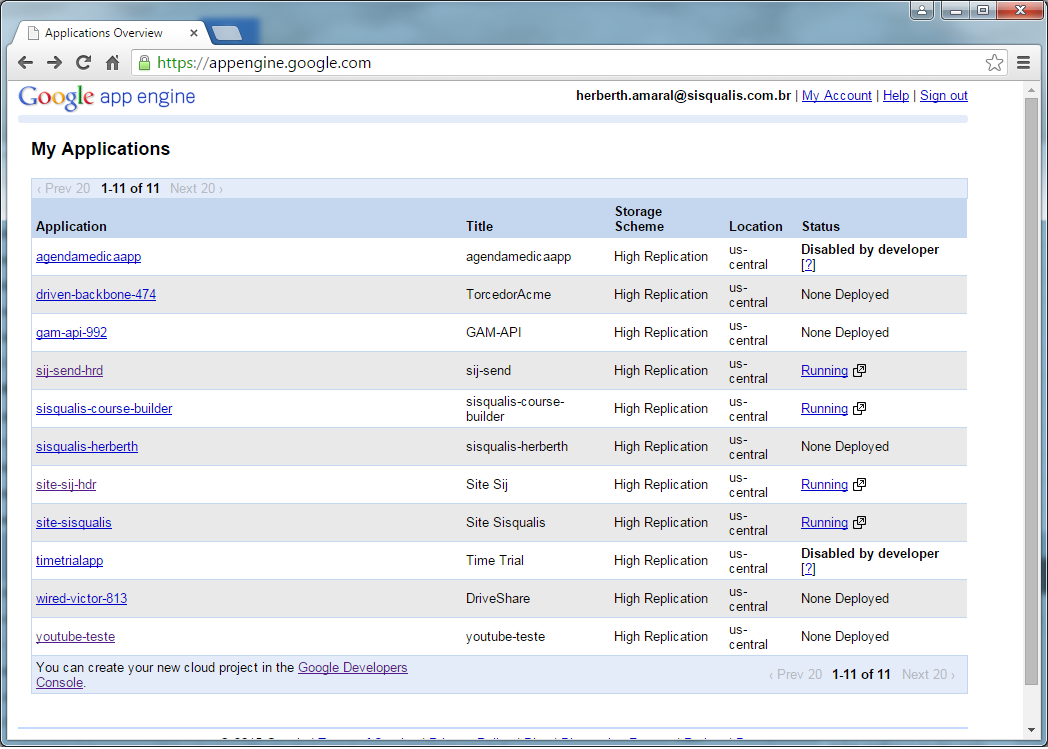
\includegraphics[width=0.75\textwidth]{painel.png}
    \caption{Página inicial do GAE (fonte própria)}
    \label{fig:painel}
\end{figure}

A figura \ref{fig:novoprojeto} mostra as configurações necessárias para criar
um projeto: apenas o nome e localização geográfica. Para uma aplicação padrão
do GAE, estas são as únicas configurações necessárias.

\begin{figure}
    \centering
    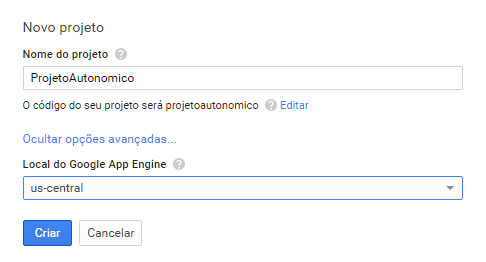
\includegraphics[width=0.75\textwidth]{novoprojeto.png}
    \caption{Interface de criação de um novo projeto no GAE (fonte própria)}
    \label{fig:novoprojeto}
\end{figure}

O painel específico de cada aplicação provê estatísticas em tempo real de
acesso, erros e outros dados de execução do projeto. A figura
\ref{fig:painel-app} mostra um exemplo do painel da aplicação. Ainda é possível
customizar o que é exibido no painel.

\begin{figure}
    \centering
    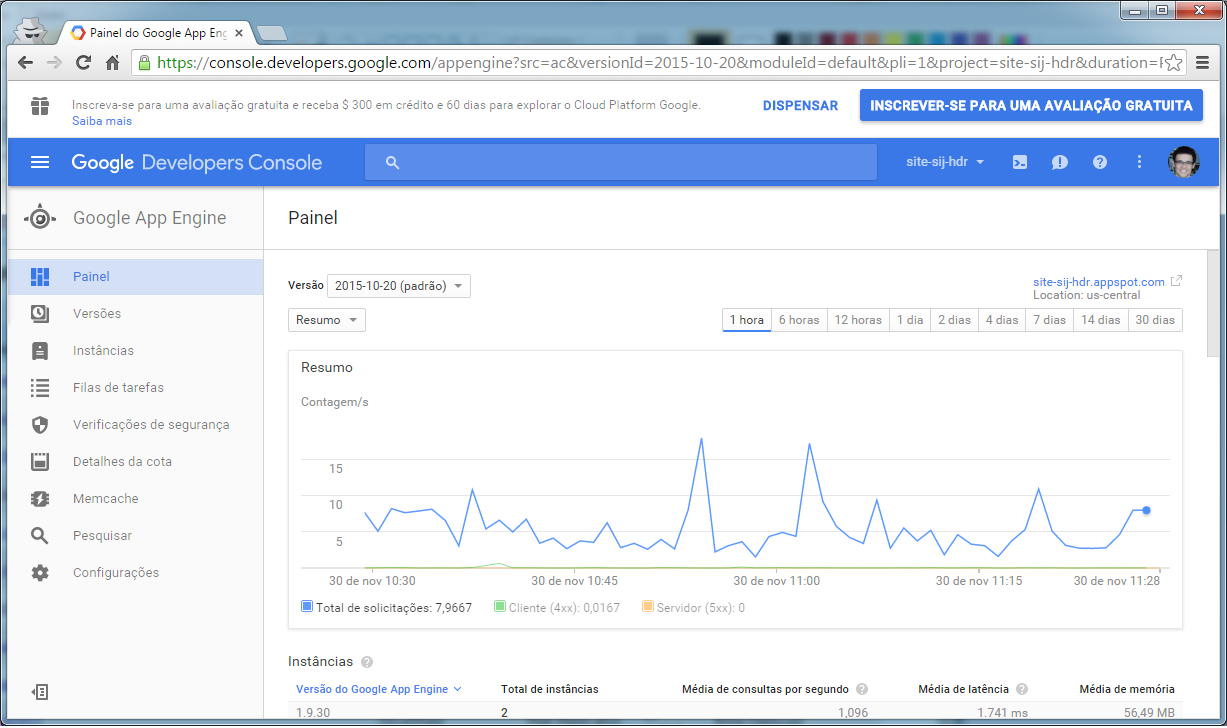
\includegraphics[width=0.75\textwidth]{painel-app.png}
    \caption{Painel específico de uma aplicação (fonte própria)}
    \label{fig:painel-app}
\end{figure}

Dependendo da carga de serviço da aplicação, o GAE provisiona novas instâncias
capazes de aumentar a capacidade de processamento das requisições extras. A
figura \ref{fig:instancias} mostra a lista de instâncias de uma aplicação em um
determinado instante.

\begin{figure}
    \centering
    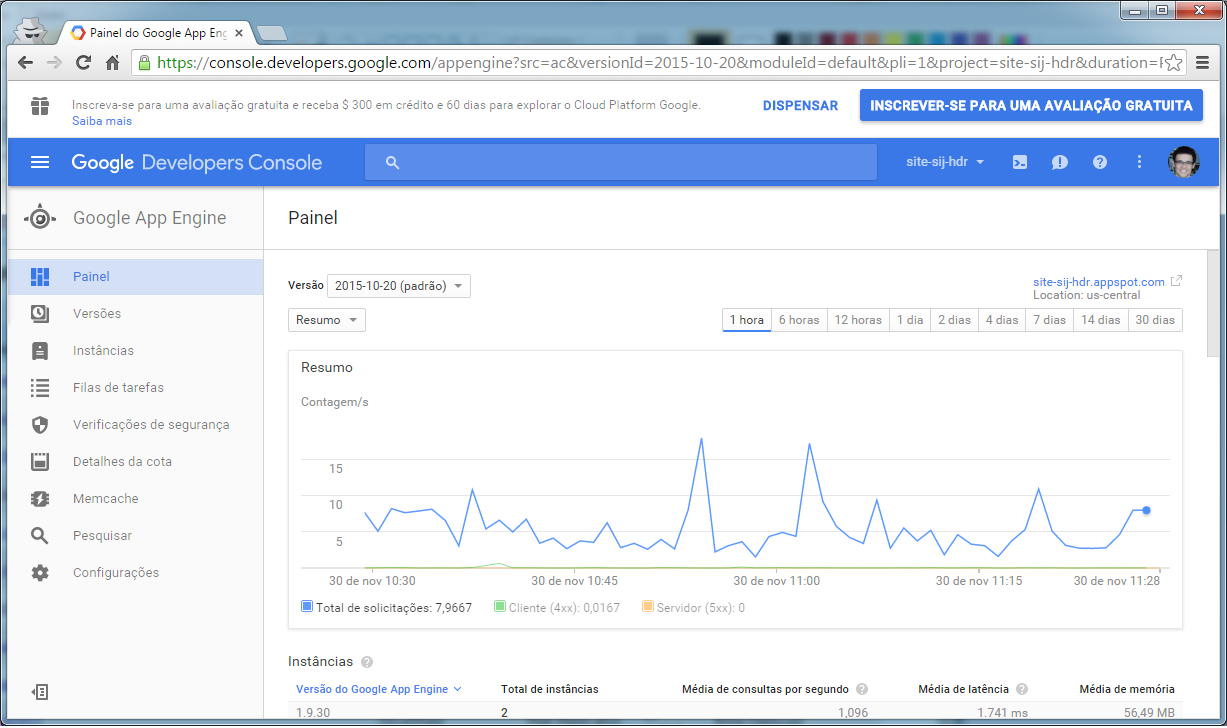
\includegraphics[width=0.75\textwidth]{painel-app.png}
    \caption{Instâncias da aplicação (fonte própria)}
    \label{fig:instancias}
\end{figure}

Por questões de segurança, o GAE mantém as versões das aplicações implantadas e
fornece a opção de intercâmbio entre elas. Um cenário de exemplo envolve uma
empresa que enviou uma versão errada e precisa voltar para a última versão.
Dependendo de como a aplicação é configurada em um servidor tradicional, esta
não pode não ser uma tarefa simples. A figura \ref{fig:versoes} mostra a
listagem das versões de uma aplicação.

\begin{figure}
    \centering
    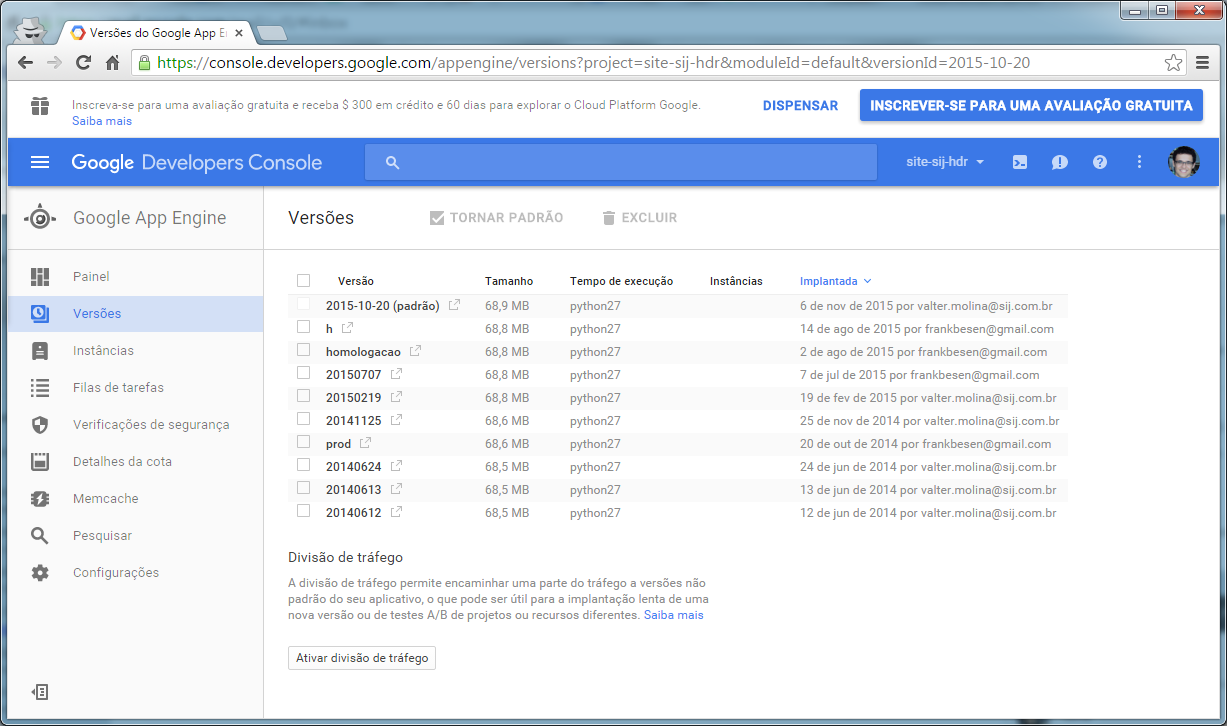
\includegraphics[width=0.75\textwidth]{versoes.png}
    \caption{Instâncias da aplicação (fonte própria)}
    \label{fig:versoes}
\end{figure}

\subsection{Serviços disponíveis}

Uma aplicação é composta de, pelo menos, uma instância que a executa. No
entanto, em cenários práticos, raramente uma aplicação é composta da instância
apenas. A seguir, lista-se os serviços básicos disponíveis no GAE para suporte
à aplicações.

\subsubsection{BigTable}

O BigTable é uma tecnologia de banco de dados do Google altamente escalável,
que permite grandes volumes armazenamento (algo da ordem de terabytes ou até
petabytes de dados) \cite{bigtable}. O BigTable também é o banco de dados
padrão do GAE.

O principal fator que permite a alta escalabilidade do BigTable é ausência de
restrições de integridade por padrão, como é comum em bancos de dados
relacionais. Por este motivo, o BigTable não é indicado para aplicações que
precisam ter um alto controle da integridade dos dados (como por exemplo,
aplicações financeiras).

Segundo \cite{bigtable}, as principais aplicações do BigTable são:
\begin{enumerate}
    \item Dados de marketing: histórico de compras e preferências de consumidores;
    \item Dados financeiros não-sensíveis, tais como histórico de transações, preço de ações e taxas de câmbio;
    \item Dados de Internet das coisas, tais como relatório de uso de medidores de energia e appliances domésticos;
    \item Dados de séries temporais, tais como uso de CPU e memória com o tempo de múltiplos servidores.
\end{enumerate}

Apesar do BigTable não ser uma opção viável para algumas aplicações, há a
possibilidade de mesclar o armazenamento de dados. Desta forma é possível
deixar os dados sensíveis em um banco de dados relacional (Google Cloud SQL) e
os dados de maior volume e sem grande importância de integridade no BigTable.

\subsubsection{CloudSQL}

O Google Cloud SQL é uma solução de banco de dados relacional completamente
gerenciado pelo Google \cite{cloudsql}. É uma alternativa ao BigTable no que
tange a segurança de integridade dos dados.

Atualmente o Google Cloud SQL só provê suporte para o sistema de gerenciamento
de banco de dados MySQL.

\subsubsection{Task Queue}

O \textit{Task Queue}, ou simplesmente fila de tarefas, é um mecanismo
disponibilizado pelo GAE para execução de tarefas demoradas para serem feitas
em uma única requisição, como a geração de relatórios complexos ou o envio de
múltiplos e-mails.

Por padrão, o tempo de execução de cada requisição é de até 60 segundos \cite{timeout}. Para
requisições acima deste tempo, há a necessidade da fila de tarefas.

\subsubsection{E-mail}

O GAE fornece uma interface de programação para envio de e-mails sem a
necessidade de configurar um servidor para tal fim \cite{mail}.

Por questões de segurança, não é possível enviar e-mails conectando-se
diretamente a um servidor SMTP na porta 25, mas é possível utilizando a porta
587 \cite{sockets}.

\subsection{Configuração dos elementos autonômicos}

Para oferecer uma boa qualidade de serviço, elementos de computação autonômica
são essenciais para o GAE. O principal motivo para essa característica é a alta
complexidade interna do GAE, que não pode ser exposta para o usuário final.

A seguir, expõe-se cada elemento da computação autonômica do GAE.

\section{Auto-cura}

O processo de auto-cura é o mais importante do GAE porque, dado a complexidade
interna do GAE, componentes falham e precisam ser restaurados ao seu estado
original.

A auto-cura do GAE compreende principalmente os seguintes pontos:

\begin{enumerate}
    \item Auto-restauração de instâncias que foram "mortas" por algum motivo;
    \item Auto-restauração de backups de bases de dados que foram corrompidas;
    \item Auto-restauração de conexões de rede;
\end{enumerate}

\section{Auto-otimização}

Alguns serviços web possuem uma rotina de acesso não-constante em que em
determinados períodos do dia há mais demanda que outros. Para efeitos de
economia, apenas o que é necessário no momento é instanciado e mais instâncias
são adicionadas à medida que a demanda aumenta. Esse recurso é conhecido como
\textit{autoscaling} \cite{autoscaling}.

Essas instâncias podem ser instâncias do servidor da aplicação, de fila de
tarefas ou de bancos de dados (no caso, somente o BigTable).


\section{Auto-proteção}

Os protocolos de auto-proteção, tais como auto-atualização da pilha de software
e uso de HTTPs por padrão, são aplicados no GAE por padrão \cite{whitepaper}. No entanto, os
protocolos básicos por si, não atendem as demandas atuais de auto-proteção de
serviços web.

O tipo de ataque mais difícil de lidar é o ataque de negação de serviço
distribuído (DDoS - \textit{distributed denial of service}), pois há várias
fontes do ataque e a classificação de um alto número de acessos para um ataque
não é trivial.

No entanto, apesar das dificuldades, o GAE oferece uma boa proteção à DDoS
através do bloqueio de acesso de regiões com alto número de requisições
sabidamente maliciosas \cite{dos}.

\section{Auto-configuração}

Na complexa infraestrutura do Google, boa parte dos parâmetros não são
configurados manualmente. Isso significa que o Google abstrai boa parte da
complexidade de configuração para seu usuário final.

URLs de bancos de dados, sistema operacional de execução, configurações de rede
e de firewall são alguns dos vários itens auto-configurados pelo GAE.

No auto-scaling também é necessário auto-configurar as novas instâncias e assim
a auto-configuração efetua um dos seus papéis fundamentais, que é permitir a
auto-cura e a auto-otimização.

\section{Considerações finais}

Este artigo procurou mostrar como os mecanismos de computação autonômica
aplicam-se no GAE. De fato, não é possível disponibilizar uma plataforma de
PaaS sem os elementos da computação autonômica, uma vez que a complexidade de
não ter um dos itens é imensa.

O mecanismo de auto-cura busca assegurar que a aplicação funcione pelo máximo
de tempo possível, independentemente das interpéries que podem acontecer.

A habilidade de escalar automaticamente é o principal componente da
auto-otimização, que é um pouco também do processo de auto-cura pelo fato que
este mecanismo busca manter a aplicação responsiva mesmo sob alta carga de
trabalho.

Os protocolos de segurança adotados pelo Google, com configurações disponíveis
para o usuário formam o componente de auto-proteção. Sem este mecanismo não
seria possível contar com nenhum outro do sistema autonômico.

\bibliographystyle{alpha}
\bibliography{artigo}

\end{document}
